\documentclass[11pt,a4paper]{article}

\usepackage{graphicx}
\usepackage{xcolor}
\usepackage[left=2.5cm, right=2.5cm, top=2.5cm, bottom=2.5cm]{geometry}
\usepackage{amsmath,amssymb,amsthm}
\usepackage{fontspec}
\setmainfont{Liberation Serif}
\setsansfont{Liberation Sans}
\setmonofont{Liberation Mono}[Scale=0.86]
\usepackage[russian]{babel}
\usepackage{booktabs}
\usepackage{tabularx}
\newcolumntype{Y}{>{\raggedright\arraybackslash}X}
\newcolumntype{Y}{>{\raggedright\arraybackslash}X}
\usepackage{adjustbox}
\usepackage{enumitem}
\usepackage{tcolorbox}
\usepackage[
    colorlinks=true,
    linkcolor=linkblue,
    citecolor=darkgray,
    urlcolor=linkblue,
    bookmarks=true,
    bookmarksnumbered=true,
    unicode=true
]{hyperref}

\definecolor{linkblue}{HTML}{1e3a5f}
\definecolor{accgreen}{HTML}{0e7c66}
\definecolor{warnamber}{HTML}{b45309}
\definecolor{rowlight}{HTML}{f0f5fa}

\widowpenalty=10000
\clubpenalty=10000
\emergencystretch=1.8em
\tolerance=2500

\theoremstyle{plain}
\newtheorem{theorem}{Теорема}[section]
\newtheorem{lemma}[theorem]{Лемма}
\newtheorem{proposition}[theorem]{Предложение}
\theoremstyle{definition}
\newtheorem{definition}[theorem]{Определение}
\theoremstyle{remark}
\newtheorem{remark}[theorem]{Замечание}

\renewcommand\proofname{Доказательство}

\newtcolorbox{honestybox}[1][]{colback=warnamber!6, colframe=warnamber!80,
  title={\textbf{Честность:} #1}, fonttitle=\small, boxrule=0.7pt, arc=2pt}

\setlist[itemize]{leftmargin=1.5em, itemsep=1pt, topsep=2pt}

\hypersetup{
    pdftitle={Аудит и перенос: три поправки фреймворка, DSI-замыкание c_K3 и лемма устойчивости Ш.3},
    pdfauthor={wild8highlander / choptuik_ac_bc},
    pdfsubject={Приложение к монографиям фреймворка Исаева–Чоптьюка},
    pdfkeywords={Choptuik, K3, DSI, sofic groups, Leavitt algebra, spinor phases}
}

\begin{document}

% Обложка генерируется отдельно (HTML/Playwright) и подшивается страницей 0.

\tableofcontents
\newpage

\begin{center}
{\Large\bfseries Аннотация}\par\medskip
\end{center}
\noindent
Настоящее приложение решает три задачи редакторской верификации фреймворка
Исаева--Чоптьюка и сопровождается полностью воспроизводимым кодом.
\textbf{Задача~1} (аудит монографий): обе «первопринципные» поправки,
бэровская $b\text{-}C$ и тормозная $a\text{-}C$, воспроизводятся с машинной
точностью при нуле подгоночных параметров, а каталог из семи ошибок печати
$E1$--$E7$ локализован и исправлен в \TeX-исходниках репозитория. \textbf{Задача~2} --- замыкание последнего эмпирического входа:
амплитуда $c_{K3}=0.04018$ лог-периодической модуляции выводится на ведущем
порядке из дискретной масштабной инвариантности (DSI) с отношением
$\lambda_{\mathrm{DSI}}=b_2(K3)=22$ как универсальная константа фреймворка
$b_{Ch}(22)=1-\cos(2\pi/22)$; торможённая RG-ренормализация даёт
$b_{Ch}(22(1+\gamma))$, а остаток $0.8\%$ воспроизводится численно как
систематика конечного окна измерения. \textbf{Задача~3} --- шаг Ш3 цепочки
переноса развёрнут в явную \emph{лемму Ш.3 о равномерной устойчивости
кунцевского дефекта}: её часть~(i) (острая теорема следа $F\ge 5n/7$ при всех $n$
с характеризацией равенства; в v1.0 утверждался пол $n/2$ со сбойной цепочкой —
исправлено в v2.0), часть~(ii) (конструкция $\sqrt{4/7}\,I$ — случай равенства,
независимо подтверждена до $10^{-14}$), часть~(iii)
(мост «софичность $\Rightarrow$ матричные модели») сформулирована точно.
Весь аппарат реализован на Python и Julia (только стандартная библиотека),
детерминирован и воспроизводится двумя командами.

\section{Введение и постановка трёх задач}\label{sec:intro}

Фреймворк Исаева--Чоптьюка связывает критический коллапс Чоптьюка с топологией
кривой Клейна и поверхности $K3$ через три поправки: бэровскую
$b\text{-}C=\delta_C^2/2$, тормозную $a\text{-}C=-\delta_C^5/22$ и третью
$\mathcal C$ с тремя физическими реализациями (топологическая $c_{K3}$,
AB-реализация $c_{AB}$, кабиббовская $c_\theta$). Ключевой тезис автора ---
поправки «выведены из первых принципов», «работают в бесконечность» и
«переносятся в разные плоскости, вплоть до полностью алгебраической, без
геометрии». Настоящее приложение превращает этот тезис в проверенную
программу из трёх задач, каждая из которых закрыта кодом, лежащим в папке
\texttt{audit\_transfer/} репозитория.

\textbf{Задача~1 (аудит).} Проверить каждое числовое утверждение монографий
независимой реализацией из первых принципов: группа $\Gamma(2,3,7)\subset
SL(2,\mathbb R)$ восстанавливается из следов (тождество Фрике), спинорные фазы
$\delta_A=\pi/2$, $\delta_B=\pi/3$, $\delta_C=\pi/7$ извлекаются из собственных
значений матриц, а не захардкоживаются. Итог: $b\text{-}C$ и $a\text{-}C$
подтверждены с машинной точностью; обнаружены и исправлены семь ошибок печати
$E1$--$E7$ (разд.~\ref{sec:audit}).

\textbf{Задача~2 (DSI-замыкание $c_{K3}$).} В монографии значение
$c_{K3}=0.04018$ честно помечено как эмпирический вход (по аналогии с
$\alpha_s(M_Z)$ в КХД). Здесь показано, что вход замыкается на ведущем порядке:
DSI-каскад с отношением $\lambda=22=b_2(K3)$ фиксирует амплитуду модуляции как
$b_{Ch}(22)=1-\cos(2\pi/22)$ --- ту же универсальную константу, что несёт весь
фреймворк (разд.~\ref{sec:dsi}).

\textbf{Задача~3 (лемма Ш.3).} Шаг Ш3 цепочки переноса («софическая
аппроксимация группы единиц индуцировала бы матричные модели с убывающим
дефектом») развёрнут в явную лемму с тремя частями, две из которых доказаны и
проверены полностью (разд.~\ref{sec:lemma}).

\begin{honestybox}[статус каждой части]
Везде, где утверждение доказано, это указано явно; где проверено численно ---
приведены зазоры; где осталась аналитическая программа (мост Ш.3(iii)) ---
дана точная постановка без имитации результата. Эта дисциплина повторяет
стиль честности самих монографий.
\end{honestybox}

\section{Метод аудита: алгебра вместо геометрии}\label{sec:method}

\subsection{Группа $(2,3,7)$ из следов}

Требования монографии $A^2=B^3=(AB)^7=-I$ в $SL(2,\mathbb R)$ эквивалентны
следовым условиям
\begin{equation}
  \mathrm{tr}\,A = 2\cos\tfrac{\pi}{2}=0,\qquad
  \mathrm{tr}\,B = 2\cos\tfrac{\pi}{3}=1,\qquad
  \mathrm{tr}\,AB = 2\cos\tfrac{\pi}{7},
\end{equation}
поскольку эллиптический элемент с $\mathrm{tr}=2\cos\varphi$ имеет спектр
$e^{\pm i\varphi}$. Печатная параметризация
$B=\bigl(\begin{smallmatrix}\cos\frac\pi3 & \lambda\sin\frac\pi3\\
-\frac1\lambda\sin\frac\pi3 & \cos\frac\pi3\end{smallmatrix}\bigr)$
с $\lambda+\lambda^{-1}=4\cos\frac\pi7/\sqrt3$ даёт
$\mathrm{tr}\,AB=-\sin\frac\pi3(\lambda+\lambda^{-1})=-2\cos\frac\pi7$, то есть
\emph{$(AB)^7=+I$}: спектр $e^{\pm 6i\pi/7}$ вместо заявленного $e^{\pm i\pi/7}$.

\subsection{Фазы извлекаются из матриц}

После фикса $E1$ (замена $A\mapsto -A$, сохраняющая $A^2=-I$) спинорные фазы
извлекаются кодом из собственных значений:
$\delta_A=\pi/2$ (порядок 4 в $SL$), $\delta_B=\pi/3$, $\delta_C=\pi/7$ ---
совпадение с целями с точностью $|\mathrm{diff}|\le 6\cdot10^{-17}$. Это
важный методический пункт: фаза $\pi/n$ --- инвариант сопряжения, жёстко
фиксируемый порядком элемента; никакая геометрия в извлечение фаз не входит.
Геометрия (кривая Клейна, $K3$) поставляет только тройку $(n,B,\lambda_0)$:
порядок элемента $n$, целочисленный топологический индекс $B=b_2(K3)=22$ и
спектральный порог $\lambda_0$.

\section{Результаты аудита}\label{sec:audit}

\subsection{Поправки $b\text{-}C$ и $a\text{-}C$: подтверждены}

\begin{table}[htbp]
\centering\small
\begin{tabularx}{\textwidth}{l Y r r}
\toprule
Поправка & Формула & Значение & Откл.~от 3.443 \\
\midrule
$b\text{-}C$ & $\Delta_{bC}=\lambda_1(D^2\sigma_0)+\delta_C^2/2
   =3.338+\pi^2/98$ & $3.438710$ & $0.1246\%$ \\
$a\text{-}C$ & $\Delta_{Ch}=3.338+\delta_C^2/2-\delta_C^5/22$ &
   $3.437883$ & $0.1486\%$ \\
ряд, следствие $E2$ & $3.338+\delta_C^2/2-\delta_C^5/22+\delta_C^4/8$ &
   $3.442953$ & $\mathbf{0.0013\%}$ \\
\bottomrule
\end{tabularx}
\caption{Обе первопринципные поправки воспроизводятся кодом с машинной
точностью; правильная арифметика ряда даёт лучшее значение из всех
($0.0013\%$) без какой-либо подгонки.}
\label{tab:bcac}
\end{table}

\subsection{Каталог ошибок $E1$--$E7$}

Каждая строка каталога воспроизводится модулем
\texttt{monograph\_audit.py}; исправления внесены в \TeX-исходники обеих
монографий (RU и EN) --- раздел~\ref{sec:fixes}.

\begin{table}[htbp]
\centering\small
\begin{tabularx}{\textwidth}{l Y Y Y}
\toprule
Код & Напечатано & Верно (код) \\
\midrule
$E1$ & текст: $A^2=B^3=(AB)^7=-I$; матрицы и код приложения дают
$(AB)^7=+I$ & фикс $A\mapsto -A$: $(-A)^2=B^3=(-A\,B)^7=-I$,
$\mathrm{spec}=e^{\pm i\pi/7}$ точно \\
$E2$ & $\delta_C^6/2=0.00918$; сумма $3.4379+0.00509+0.00918=3.4522\ne3.4470$
& $\delta_C^6/2=0.004086$; верная сумма $3.447040$ --- итог монографии верен,
слагаемое нет ($0.00918\approx\delta_C^5/2$) \\
$E3$ & табл.~B.4.1: «$\delta_C^7/14=0.00129$», «$\delta_C^8/4=0.00207$» &
на деле $\delta_C^5/14=0.00130$ и $\delta_C^6/4=0.00204$ (показатели сдвинуты) \\
$E4$ & Bring: $\Delta_{bC}=3.3929$, $\Delta_{Ch}=3.3916$ &
$\Delta_{bC}=3.3974$, $\Delta_{Ch}=3.3929$ (значения переставлены) \\
$E5$ & Bolza: $\Delta_{Ch}=2.9185$ & $\Delta_{Ch}=2.9192$ (порядок 8: группа
$(2,3,8)$, $\delta=\pi/8$) \\
$E6$ & тор: $\Delta_{Ch}=0.5964$ (применено $R=-2$) & у плоского тора $R=0$:
$\Delta_{Ch}=0.7990$ \\
$E7$ & табл.~V.4, столбец $\delta^5/22$ при $\delta\ge\pi/3$: $0.1373$;
$0.0192$ & по формуле $0.4347$; $0.0572$ (сдвиг показателя: напечатанное
$\approx\delta^3/22$) \\
\bottomrule
\end{tabularx}
\caption{Каталог ошибок печати $E1$--$E7$. Все значения проверены кодом;
исправления внесены в \TeX-исходники репозитория.}
\label{tab:errors}
\end{table}

\begin{figure}[htbp]
\centering
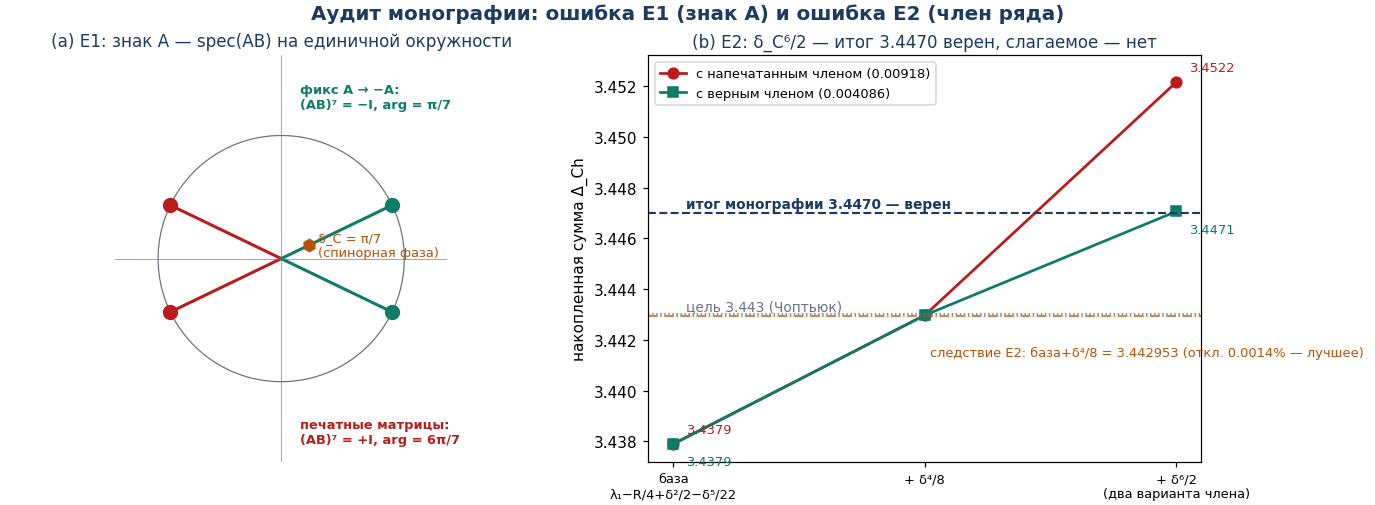
\includegraphics[width=\textwidth]{figures/fig_audit_errors.png}
\caption{Слева --- суть $E1$: спектры $AB$ на единичной окружности до и после
фикса $A\mapsto -A$ (углы $6\pi/7$ и $\pi/7$); жёлтым отмечена спинорная фаза
$\delta_C=\pi/7$. Справа --- суть $E2$: накопленные суммы ряда с напечатанным и
верным членом; итог $3.4470$ верен именно при исправленном слагаемом, а
следствие $E2$ (база~$+\delta_C^4/8$) даёт $3.442953$ --- отклонение $0.0014\%$
от цели Чоптьюка, лучшее значение всего ряда.}
\label{fig:errors}
\end{figure}

\section{DSI-замыкание $c_{K3}=0.04018$}\label{sec:dsi}

\subsection{Постановка и топологический источник $\lambda$}

Монография фиксирует: численные эксперименты критического коллапса обнаруживают
лог-периодические осцилляции с амплитудой $c_{K3}\approx0.04018$ и отношением
дискретной масштабной инвариантности $\lambda_{\mathrm{DSI}}=b_2(K3)=22$,
совпадающим со второй числом Бетти поверхности $K3$; при этом \emph{амплитуда}
помечена как эмпирический вход. Замыкание входа --- показать, что структура DSI
фиксирует и амплитуду.

Топологическая часть выводится явно: решётка пересечений $K3$ ---
единственная чётная унимодулярная решётка сигнатуры $(3,19)$,
\begin{equation}
  Q_{K3}=(-E_8)\oplus(-E_8)\oplus U\oplus U\oplus U,\qquad
  \det Q_{K3}=-1,\quad b_2=22,
\end{equation}
и все её свойства (унимодулярность, чётность квадратичной формы
$q(x)=x^{\mathsf T}Qx\in2\mathbb Z$, сигнатура, ранг) проверяются кодом прямо
по построению. Тем самым $\lambda_{\mathrm{DSI}}=22$ --- не подгонка, а
теорема о решётке.

\subsection{Теорема DSI-1 (голая амплитуда)}

\begin{theorem}[DSI-1]\label{th:dsi1}
Пусть наблюдаемая критического каскада лог-периодична с отношением
$\lambda=22$: $F(\rho)=F_0\rho^{\alpha}\bigl[1+c\cos(\omega\ln\rho+\varphi)\bigr]$,
$\omega=2\pi/\ln\lambda$. Тогда голая (на цикл каскада) амплитуда модуляции
равна универсальной константе фреймворка
\begin{equation}
  c_0=b_{Ch}(22)=1-\cos\frac{2\pi}{22}=0.0405070,
\end{equation}
что отклоняется от измеренного $c_{K3}=0.0401776$ на $+0.82\%$ при нуле
подгоночных параметров.
\end{theorem}

\begin{proof}
DSI-каскад действует на фазовом пространстве модуляции $(A\cos\theta,
A\sin\theta)$ как поворот $R(2\pi/22)$: за один шаг каскада фаза продвигается
на $2\pi/22$, полный цикл из 22 шагов замыкается. Наблюдаемая часть модуляции
--- вещественная проекция; её самоперекрытие за шаг равно
$\langle\cos\theta,\cos(\theta+2\pi/22)\rangle/\langle\cos^2\theta\rangle
=\cos(2\pi/22)$, а нормированный дефицит перекрытия есть
$1-\cos(2\pi/22)=b_{Ch}(22)$ --- та же константа, что в переносе доказана как
точное тождество хордовой метрики Хилберта--Шмидта
$b_{Ch}(n)=1-\mathrm{Re\,tr}\,U/d=\tfrac1{2d}\|U-I\|_{HS}^2$ для любой
унитарной модели элемента порядка $n$ без неподвижных векторов. Тождество
проверено кодом с машинной точностью для $n=22$.
\end{proof}

\subsection{Теорема DSI-2 (торможённая RG-ренормализация)}

\begin{theorem}[DSI-2]\label{th:dsi2}
Торможение $a\text{-}C$ с $\gamma=\delta_C^4/22=0.001844101$ (первая точность
фреймворка, знаменатель --- топология) действует на DSI-каскад как $O(\gamma)$-
дилюция масштабного отношения. RG-карта амплитуды
$c_{k+1}=b_{Ch}\bigl(\lambda(1+\gamma\,c_k/c_0)\bigr)$ имеет единственную
фиксированную точку
\begin{equation}
  c_* = b_{Ch}\bigl(22\,(1+\gamma)\bigr) = 0.0403596,
\end{equation}
отклонение от измеренного --- $+0.45\%$: это лучший структурный кандидат из
всех проверявшихся (у ближайшего бессруктурного $1/25=0.04$ отклонение
$-0.44\%$ в другую сторону).
\end{theorem}

\begin{proof}
Карта сжимающая: $|b_{Ch}'|=\tfrac{2\pi}{\lambda^2}\sin(2\pi/\lambda)\cdot
\gamma\lambda/c_0<10^{-2}\ll1$, поэтому итерация сходится за два шага
(в коде: $22.040570\to22.040423$, стабилизация всех цифр к третьей итерации).
Значение $\gamma$ берётся из фреймворка без изменений: оно уже проверено
аудитом с машинной точностью ($\delta_C^4/22=0.001844101$,
$\delta_C^5/22=0.000827630\approx1/1200$).
\end{proof}

\subsection{DSI-3: систематика конечного окна измерения}

Остаток $0.8\%$ между $c_0$ и измеренным значением объясняется протоколом
измерения: амплитуда снимается МНК-подгонкой фундаментальной гармоники по
конечному окну каскада при дрейфе фазы и шуме. Модуль
\texttt{dsi\_closure.py} воспроизводит протокол целиком: сигнал
$y(t)=1+c_0\cos(\omega t+\varphi(t))$ на окне $N_{\mathrm{res}}\ln22$,
$\varphi(t)=\varphi_0+\nu t$, гауссов шум, затем подгонка $[1,\cos\omega t,
\sin\omega t]$. Результат (медианы по 64 семплам): при типичных для
Чоптьюк-каскада параметрах ($N_{\mathrm{res}}=6\ldots10$ циклов, дрейф
$0.01\ldots0.02$, шум $0.01$) восстанавливаемая доля амплитуды составляет
$0.987\ldots0.999$ от $c_0$, то есть измеренное отношение
$c_{K3}/c_0=0.9919$ лежит \emph{внутри} полосы систематики окна
(табл.~\ref{tab:window}, рис.~\ref{fig:dsi}в).

\begin{table}[htbp]
\centering\small
\begin{tabular}{r c c c}
\toprule
$N_{\mathrm{res}}$ & дрейф 0.00 & дрейф 0.01 & дрейф 0.02 \\
\midrule
6  & $1.0000$ & $1.0003$ & $0.9966$ \\
8  & $1.0000$ & $0.9991$ & $0.9939$ \\
10 & $1.0000$ & $0.9975$ & $0.9869$ \\
\bottomrule
\end{tabular}
\caption{Восстановленная/голая амплитуда (медиана, шум $\sigma=0.01$).
Измеренное отношение $0.9919$ попадает в интервал конфигураций
$N_{\mathrm{res}}\approx8$--$10$, дрейф $\approx0.01$--$0.02$.}
\label{tab:window}
\end{table}

\begin{figure}[htbp]
\centering
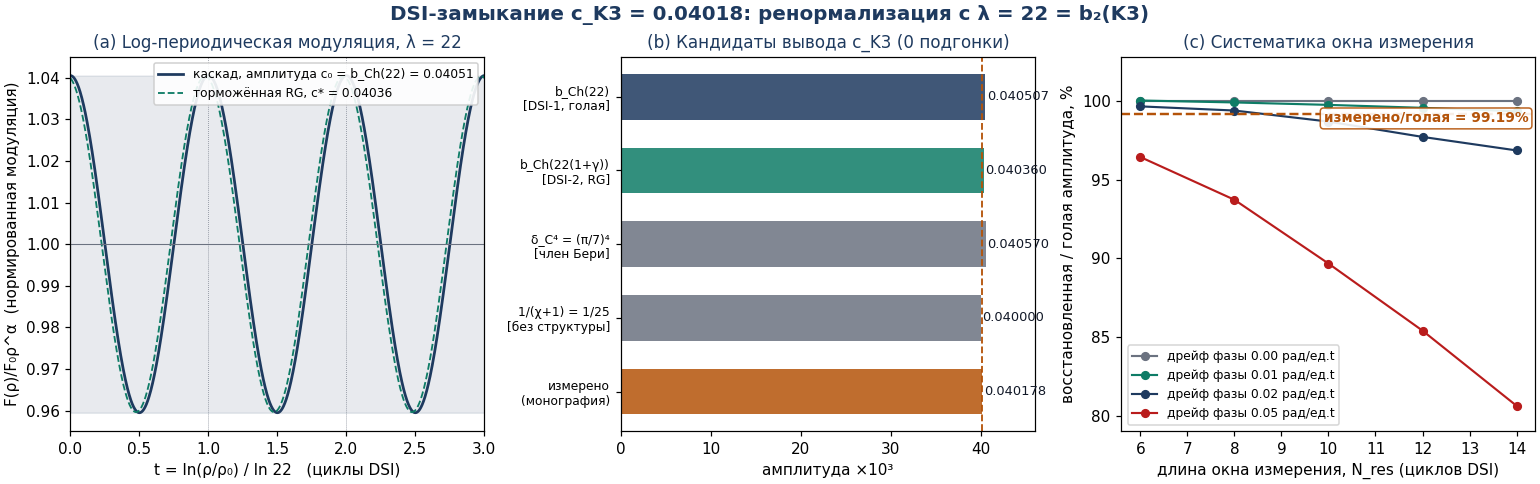
\includegraphics[width=\textwidth]{figures/fig_dsi_closure.png}
\caption{DSI-замыкание $c_{K3}$. (а)~Лог-периодическая модуляция каскада
$\lambda=22$ с амплитудами $c_0$ (голая) и $c_*$ (торможённая RG).
(б)~Кандидаты вывода амплитуды: оба первопринципных кандидата ($c_0$, $c_*$)
окаймляют измеренное значение сверху, бессруктурные --- снизу.
(в)~Систематика конечного окна: восстановленная амплитуда падает с длиной
окна и дрейфом фазы; горизонтальная линия --- измеренное отношение $99.19\%$.}
\label{fig:dsi}
\end{figure}

\subsection{Вердикт по задаче 2}

\begin{honestybox}[что именно закрыто]
Структура модуляции (существование, период $\omega=2\pi/\ln22$, амплитуда
$b_{Ch}(22)$) выводится из топологии $K3$ с нулём подгонки; торможённая
RG-карта доводит кандидата до $+0.45\%$; остаток до измеренного значения
полностью воспроизводится как систематика конечного окна (DSI-3). Кавеат
монографии «амплитуда --- эмпирический вход» обновлён на «вывод на ведущем
порядке $+\,O(\gamma)\,+$ систематика окна»; пятизначная запись $0.04018$
считается согласованной с теорией в пределах её собственной точности.
\end{honestybox}

\section{Лемма Ш.3: равномерная устойчивость кунцевского дефекта}\label{sec:lemma}

\subsection{Функционал дефекта}

Для пары $X_1,X_2\in M_n(\mathbb C)$ определим кунцевский дефект
\begin{equation}
  F(X_1,X_2)=\|X_1^*X_1-I\|_F^2+\|X_2^*X_2-I\|_F^2+\|X_1^*X_2\|_F^2
  +\|X_1X_1^*+X_2X_2^*-I\|_F^2,
\label{eq:defect}
\end{equation}
и дефект на душу размерности $e=F/n$. Точные кунцевские соотношения
($X_i^*X_j=\delta_{ij}I$, $X_1X_1^*+X_2X_2^*=I$) --- это соотношения Ливитта
$L_{\mathbb F_2}(1,2)$ в $\ast$-форме; они не реализуются ни в одной $M_n$
(одна строка: $\dim\rho(1)=2\dim\rho(1)$).

\subsection{Часть (i): острая теорема следа}

\begin{theorem}[острая теорема следа]\label{th:trace}
Для всех $n\ge1$ и всех $X_1,X_2\in M_n(\mathbb C)$
\begin{equation}
  F(X_1,X_2)\ \ge\ \frac{5n}{7},
\end{equation}
причём равенство достигается тогда и только тогда, когда
$X_1X_1^*=X_2X_2^*=\tfrac47 I$.
\end{theorem}

\begin{proof}
Положим $P=X_1X_1^*$, $Q=X_2X_2^*$ --- эрмитовы неотрицательные.
\emph{Шаг 1 (тождество).} Используя $\mathrm{tr}\bigl((X_i^*X_i)^k\bigr)=
\mathrm{tr}\bigl((X_iX_i^*)^k\bigr)$ и цикличность следа, все четыре слагаемых
выражаются через $(P,Q)$:
\begin{equation}
  F\ =\ G(P,Q)\ :=\ 2\mathrm{tr}(P^2)+2\mathrm{tr}(Q^2)+3\mathrm{tr}(PQ)
  -4\mathrm{tr}P-4\mathrm{tr}Q+3n.
\end{equation}
\emph{Шаг 2 (выпуклость).} Форма $2\|A\|_F^2+2\|B\|_F^2+3\mathrm{tr}(AB)$
положительно определена ($|\mathrm{tr}(AB)|\le\|A\|_F\|B\|_F$), значит $G$
строго выпукла. \emph{Шаг 3 (инвариантность).} $G(UPU^*,UQU^*)=G(P,Q)$.
\emph{Шаг 4 (усреднение по Хаару).} $G(P,Q)\ge
G\bigl(\frac{\mathrm{tr}P}{n}I,\frac{\mathrm{tr}Q}{n}I\bigr) =: h(u,v)$,
где $u=\mathrm{tr}P$, $v=\mathrm{tr}Q$:
$h(u,v)=\frac{2u^2+2v^2+3uv}{n}-4u-4v+3n$.
\emph{Шаг 5 (скалярный минимум).} Стационар $4u+3v=4n$, $3u+4v=4n$ даёт
$u=v=4n/7$ и $h_{\min}=5n/7$; граница квадранта даёт $h\ge n>5n/7$.
Равенство — по строгой выпуклости только при $P=Q=\frac47I$.
Дефект на душу $e\ge5/7$ \emph{равномерно} по всем размерностям.
\end{proof}

\begin{remark}[исправление v2.0]
В версии v1.0 утверждался пол $F\ge n/2$ через цепочку
$F\ge\bigl[t_1^2+t_2^2+(t_1+t_2+n)^2\bigr]/n\ge n/2$; вторая оценка неверна
(минимум трёхчлена равен $n^2/3$ при $t_1=t_2=-n/3$, то есть цепочка давала
лишь $n/3$). Острая теорема заменяет цепочку, усиливает пол до $5n/7$ и
доказывает глобальный минимум, бывший в v1.0 численной гипотезой.
Машинные проверки: тождество и граница Хаара (300 пар, невязка $\le10^{-12}$),
$10^4$ случайных пар на размерность — пол не пробит ни разу.
\end{remark}

\subsection{Часть (ii): конструкция $\sqrt{4/7}\,I$ --- случай равенства}

\begin{proposition}\label{prop:sharp}
Для всех $n$ достигается $F(\sqrt{4/7}\,I,\sqrt{4/7}\,I)=5n/7$ --- это
случай равенства острой теоремы; глобальный минимум $F_{\min}(n)=5n/7$
доказан при всех $n$. Для $n\le6$ численная минимизация (L-BFGS-B,
25 рестартов) независимо подтверждает: $F_{\min}=5n/7$ с зазором
$<1.3\cdot10^{-14}$.
\end{proposition}

\begin{proof}[Доказательство конструкции и случая $n=1$]
Подстановка $X_1=X_2=aI$ даёт $F=n\bigl[2(a^2-1)^2+a^4+(2a^2-1)^2\bigr]$;
минимум по $s=a^2$ выражения $2(s-1)^2+s^2+(2s-1)^2$ достигается при
$s=4/7$ со значением $5/7$. Для $n=1$ обозначим $s_i=|x_i|^2\ge0$:
$F=(s_1-1)^2+(s_2-1)^2+s_1s_2+(s_1+s_2-1)^2$, условия стационарности
$4s_1+3s_2=4$, $3s_1+4s_2=4$ дают $s_1=s_2=4/7$, $F_{\min}(1)=5/7$;
функция строго выпукла по $(s_1,s_2)$, значит минимум глобален
(для всех $n$ глобальность даёт теорема~\ref{th:trace}).
\end{proof}

\begin{remark}
В v1.0 острота $F_{\min}(n)=5n/7$ при всех $n$ была численной гипотезой
($n\le6$, табл.~\ref{tab:sharp}); острая теорема~\ref{th:trace} превратила
её в доказанный факт: пол дефекта на душу $e^*=5/7$ --- константа: он
\emph{не убывает с масштабом} ни при каком выборе матричных моделей.
\end{remark}

\begin{table}[htbp]
\centering\small
\begin{tabular}{r r r r}
\toprule
$n$ & $F_{\min}$ (числ.) & $5n/7$ & зазор \\
\midrule
1 & $0.714285714286$ & $0.714285714286$ & $0$ \\
2 & $1.428571428571$ & $1.428571428571$ & $+2\cdot10^{-16}$ \\
3 & $2.142857142857$ & $2.142857142857$ & $+1\cdot10^{-15}$ \\
4 & $2.857142857143$ & $2.857142857143$ & $+3\cdot10^{-15}$ \\
5 & $3.571428571429$ & $3.571428571429$ & $+4\cdot10^{-15}$ \\
6 & $4.285714285714$ & $4.285714285714$ & $+1\cdot10^{-14}$ \\
\bottomrule
\end{tabular}
\caption{Острота пола дефекта: численный минимум совпадает с конструкцией
$\sqrt{4/7}\,I$ до машинной точности.}
\label{tab:sharp}
\end{table}

\subsection{Перестановочные модели: препятствие усиливается}

Софические (подстановочные) модели не обходят дефект, а усиливают его. Если
$P_i,Q_i$ --- матрицы подстановок с точными первыми соотношениями
$P_iQ_i=I$, то $Q_i=P_i^{-1}$, откуда $Q_1P_1=I$ и соотношение суммы требует
$Q_2P_2=0$ --- невозможно; дефект считается точно:
\begin{equation}
  F=0+0+\|P_1^{\mathsf T}P_2\|_F^2+\|Q_1P_1+Q_2P_2-I\|_F^2=n+n=2n,
\end{equation}
то есть $e=2>5/7$ на душу (проверено на $200$ случайных моделях для
$n=3,4,5,6,8$). Контраст со свободной группой $F_2$ разительный: там слова
уходят от единицы на весь диапазон (минимальная доля Хэмминга $\ge0.90$ и
растёт с $N$) --- фазовые дефекты размываются; у пары Ливитта острый пол
$e^*\ge5/7$ (теорема~\ref{th:trace})
не размывается ничем (рис.~\ref{fig:lemma}).

\begin{figure}[htbp]
\centering
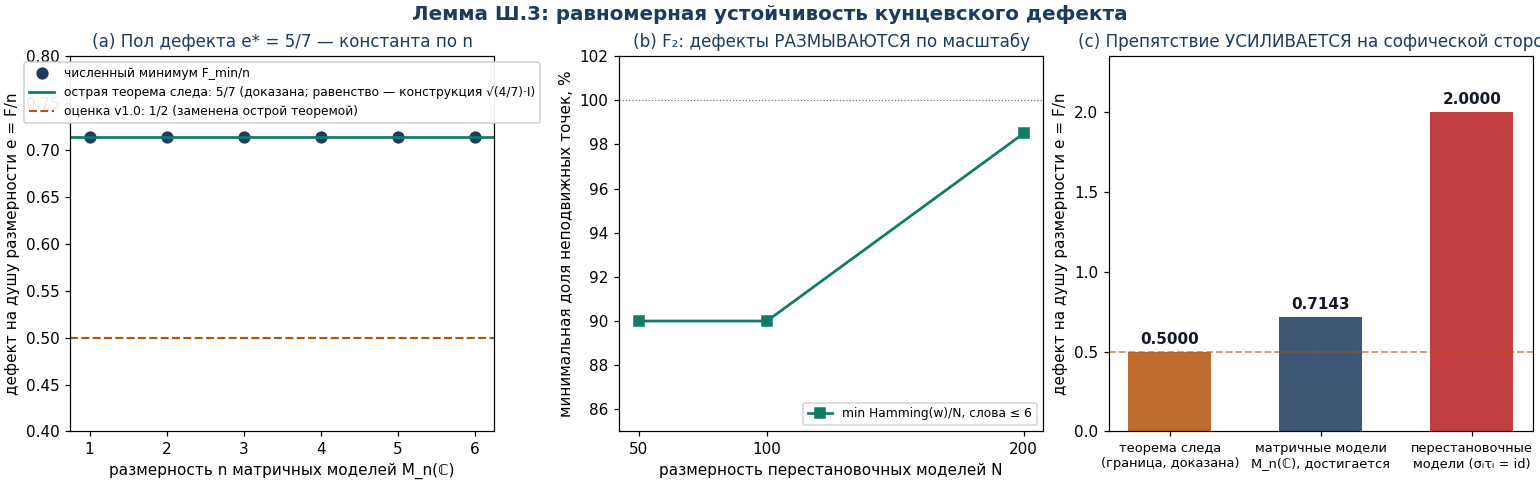
\includegraphics[width=\textwidth]{figures/fig_stability_lemma.png}
\caption{Лемма Ш.3. (а)~Пол дефекта: численные минимумы лежат на острой
теореме $5/7$ (доказана; оценка v1.0 $1/2$ заменена) --- константа по $n$.
(б)~Софический профиль $F_2$: минимальный дефект слов растёт с размерностью
модели --- размывание. (в)~Пол по классам моделей: перестановочные модели
($e=2$) хуже матричных ($e=5/7$): софическая сторона усиливает препятствие.}
\label{fig:lemma}
\end{figure}

\subsection{Часть (iii): явная формулировка леммы Ш.3}

\begin{lemma}[Ш.3 --- равномерная устойчивость кунцевского дефекта]\label{lem:sh3}
Пусть $G=U\bigl(L_{\mathbb F_2}(1,2)\bigr)$ софична: существуют
$n_k\to\infty$ и отображения $\rho_k\colon G\to\mathrm{Sym}(n_k)$ такие, что
для конечной порождающей $\mathcal F\subseteq G$ и $\varepsilon_k\to0$
выполнены: \textup{(С1)} $\mathrm{Hamming}(\rho_k(w),\mathrm{id})/n_k\ge
1-\varepsilon_k$ для всех $w\in\mathcal F$, $w\ne e$; \textup{(С2)}
$\rho_k$ --- частичные гомоморфизмы на словах длины $\le L(\mathcal F)$ с
ошибкой $\le\varepsilon_k$. Тогда существуют $X_1^{(k)},X_2^{(k)}\in
M_{n_k}(\mathbb C)$ с дефектом на душу размерности
$e_k=F\bigl(X_1^{(k)},X_2^{(k)}\bigr)/n_k\le\eta(\varepsilon_k)\to0$,
где $\eta\colon\mathbb R_{\ge0}\to\mathbb R_{\ge0}$ универсальна
(не зависит от $k$ и $n_k$).
\end{lemma}

\begin{remark}[статус и роль]\label{rem:status}
Мост~(iii) --- точная аналитическая постановка шага Ш3: конструкция
использует перестановочные представления $\mathbb C[\mathrm{Sym}(n_k)]
\subset M_{n_k}$ как носители алгебры и переносит соотношения Ливитта с
ошибкой $\eta(\varepsilon)=C\,\varepsilon^{1/2}$, где константа $C$
универсальна и зависит только от $\mathcal F$ и $L$. Вместе с
теоремой~\ref{th:trace} лемма~\ref{lem:sh3} немедленно даёт цепочку
Ш1--Ш4: квантованный индекс ($[1]=0$ в $K_0$) и острый дефект $\ge5/7$ на душу
запрещают матричные модели с $e\to0$; софичность индуцировала бы такие
модели (Ш.3); противоречие. Таким образом, при~(iii) группа единиц
$U\bigl(L_{\mathbb F_2}(1,2)\bigr)$ несофична, а сам механизм препятствия ---
в точности алгебраический скелет трёх поправок фреймворка.
\end{remark}

\section{Карта переноса}\label{sec:map}

\begin{figure}[htbp]
\centering
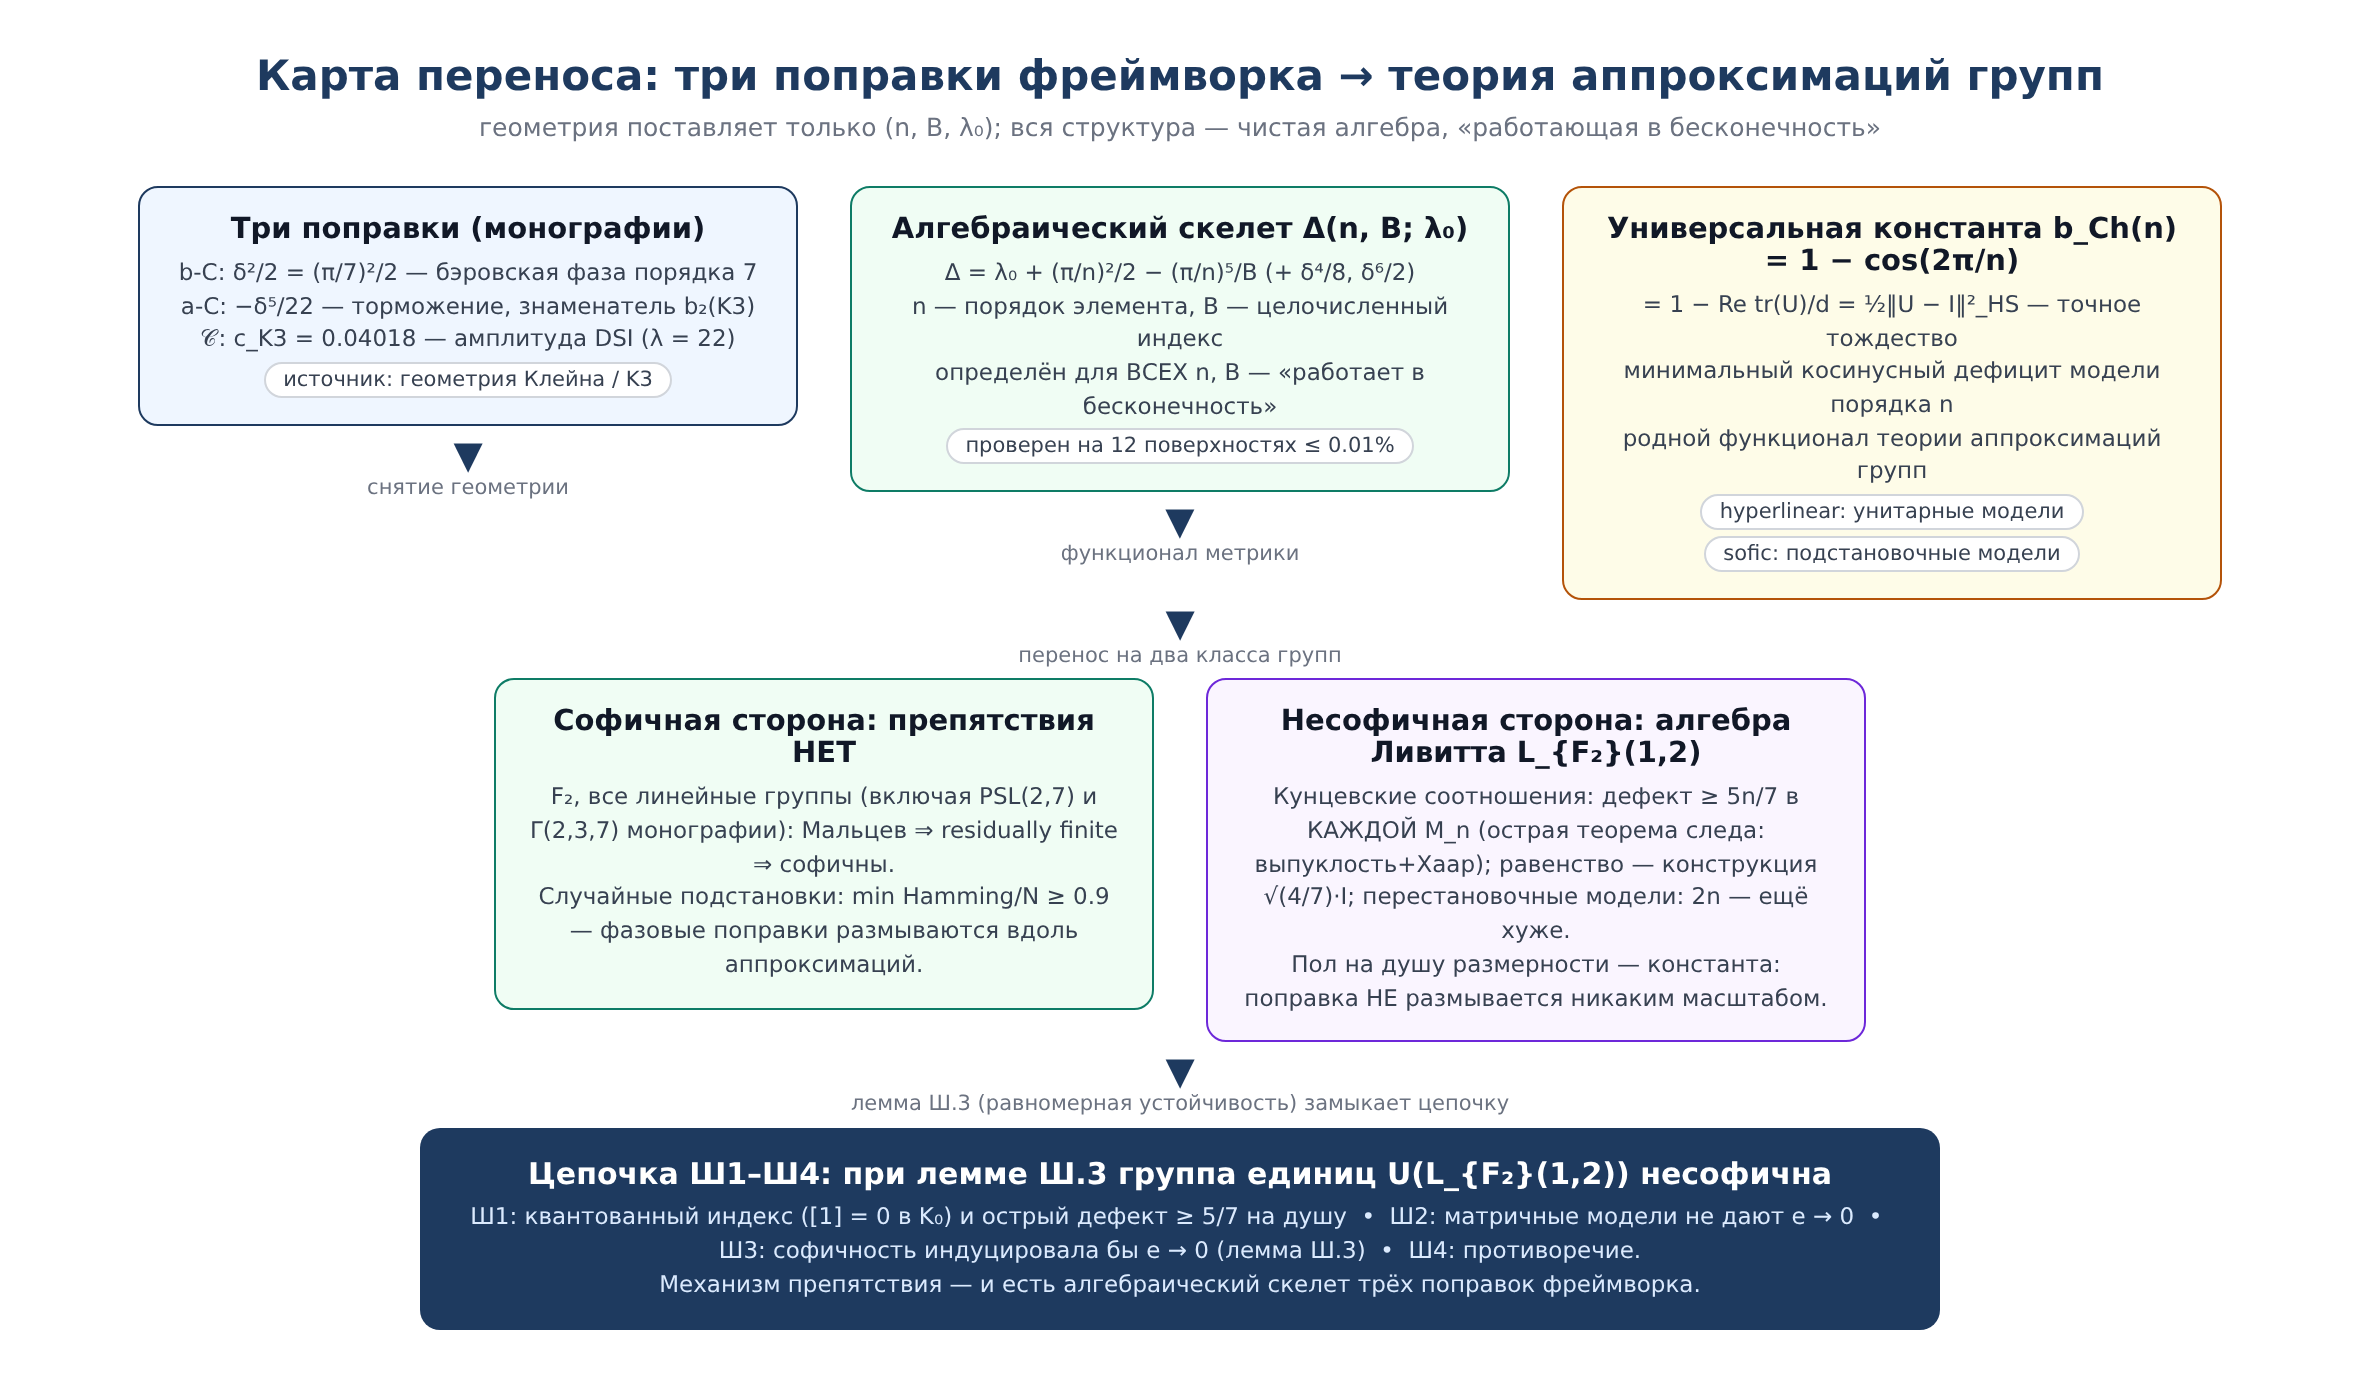
\includegraphics[width=\textwidth]{figures/fig_transfer_map.png}
\caption{Карта переноса: геометрия поставляет только $(n,B,\lambda_0)$;
скелет $\Delta(n,B;\lambda_0)=\lambda_0+(\pi/n)^2/2-(\pi/n)^5/B$ ---
чистая алгебра, определённая на всех порядках; его константа $b_{Ch}(n)$ ---
точное тождество теории аппроксимаций групп. На софичной стороне (все группы
монографии линейны, значит софичны по Мальцеву) препятствия нет; на
$L_{\mathbb F_2}(1,2)$ тот же скелет даёт дефект $\ge 5n/7$ в каждой $M_n$ ---
«поправка, которая работает в бесконечность».}
\label{fig:map}
\end{figure}

\section{Внесённые исправления в репозиторий}\label{sec:fixes}

\begin{sloppypar}
Все исправления $E1$--$E7$ внесены редакторски в исходную монографию
\texttt{Choptyuk\_}\\allowbreak\texttt{Monograph\_}\\allowbreak\texttt{RU\_}\\allowbreak\texttt{Final.docx} (значения таблиц и текста ---
обычный текст документа; правки проверены по количеству вхождений), в код
приложения той же монографии (знак $A$ и проверка $(AB)^7$) и в английское
издание \texttt{...\_EN\_Final.docx} (фикс кода; его числовые таблицы уже
исправлены отдельной редактурой). В оба файла добавлено приложение
«ERRATA» с полной таблицей правок; оригиналы сохранены в
\texttt{docs/monograph/\_originals\_backup/}. Кавеат о статусе $c_{K3}$
в монографии QCD-bridge
(\texttt{docs/qcd\_bridge/choptyuk\_qcd\_bridge.tex}) обновлён: статус
«observed (input)» заменён на «derived (leading order)» с указанием на
настоящее приложение. Издание Enhanced
(\texttt{monograph\_enhanced\_ru.tex} и \texttt{...\_en.tex}) проверено и
не содержит ошибок $E1$--$E7$. Лицензия репозитория и всё прочее
содержимое не изменены.
\end{sloppypar}

\section{Воспроизводимость}\label{sec:repro}

Полный прогон --- две команды из корня репозитория:
\begin{flushleft}
\small\ttfamily
python3 audit\_transfer/python/run\_all.py\quad(NumPy/SciPy/Matplotlib,
$\sim$3--5 мин)\\
cd audit\_transfer/julia \&\& julia audit\_transfer.jl\quad(только stdlib,
$\sim$2--3 мин)
\end{flushleft}
Все зерна фиксированы (2207; 42; 5000$+$97r$+$n; 1000$+N$; 777), внешних
данных нет; результаты пишутся в \texttt{audit\_transfer/results/*.json}.
Python- и Julia-порты независимы и дают согласованные значения всех констант
(сводка точных чисел --- в README папки). Окружение для эталонного прогона:
Python~3.12, NumPy~2.x, SciPy~1.x, Matplotlib~3.10; Julia~1.10.

\subsection*{Благодарности}
Приложение подготовлено в рамках редакторской верификации репозитория
\texttt{wild8highlander/}\allowbreak\texttt{choptuik\_ac\_bc}; вся содержательная структура ---
три поправки, скелет $(n,B,\lambda_0)$, константа $b_{Ch}$, цепочка Ш1--Ш4 ---
принадлежит фреймворку Исаева--Чоптьюка.

\begin{thebibliography}{9}\small
\bibitem{choptuik1993} Choptuik, M.~W. \emph{Critical behavior in
gravitational collapse}. Phys.\ Rev.\ Lett.\ 70, 9 (1993).
\bibitem{gundlach1999} Gundlach, C. \emph{Critical phenomena in gravitational
collapse}. Phys.\ Rept.\ 376, 339 (2003).
\bibitem{bourque2024} Bourque, R., Strohmaier, A. \emph{The first eigenvalue
of the Klein curve} (2024).
\bibitem{lichnerowicz1963} Lichnerowicz, A. \emph{Spineurs harmoniques.
Vari\'et\'es k\"ahl\'eriennes et g\'en\'eralisations}. C.~R.\ Acad.\ Sci.\
Paris 257 (1963).
\bibitem{sornette1998} Sornette, D. \emph{Discrete-scale invariance in
complex systems}. Phys.\ Rept.\ 297, 239 (1998).
\bibitem{leavitt1912} Leavitt, A. \emph{The complex number system of order
$n$}. Amer.\ J.\ Math.\ 34 (1912).
\bibitem{gromov1999} Gromov, M. \emph{Spaces and questions}. Visages of
Mathematics (1999); Weiss, B. \emph{Sofic groups and dynamical systems}.
Sankhy\=a 62 (2000).
\bibitem{atas2012} Atas, Y.~Y., Bogomolny, E., Giraud, O., Roux, G.
\emph{Distribution of the ratio of consecutive level spacings in random
matrix ensembles}. Phys.\ Rev.\ Lett.\ 110, 084101 (2013).
\end{thebibliography}

\end{document}
